\section{Introduction}
\subsection{Background}
The Corporate Partnership Program is a website designed to `promote the relationship between the Department of Computing and organisations who wish to recruit our students whilst investing in academic sponsorship'\cite{doc-cpp}.

In order for students to use the system they must log on, register some tick box interests, and then upload their CV.
For the student once they have done this their CPP journery is complete.
Corporate Partners then log on and can browse this list of students in order to contact them regarding internships, placements, and graduate oppourtunities.

\begin{figure}[H]\centering
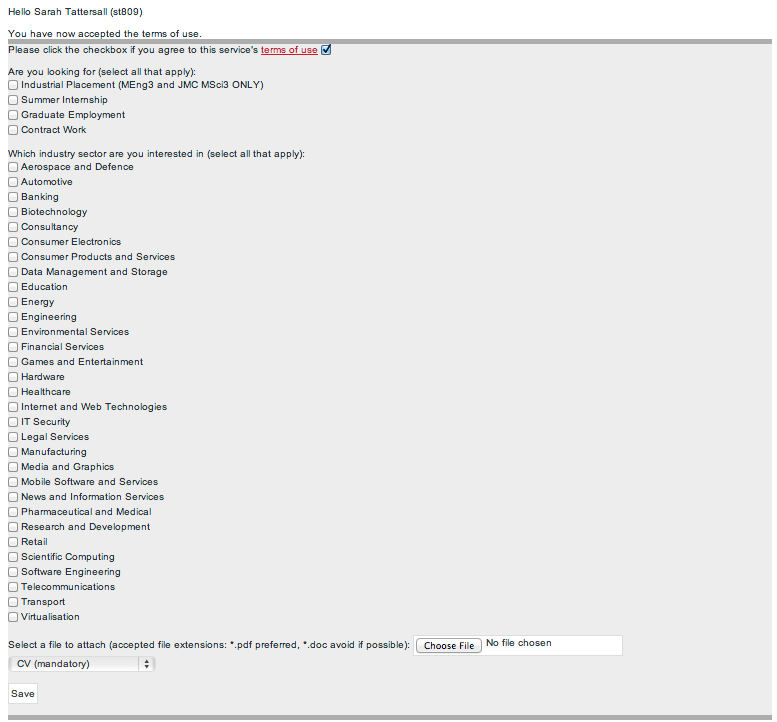
\includegraphics[scale=0.5]{images/introduction/old_cpp}
\caption{Entirety of the old site as viewable to the student}
\end{figure}


The current system has other flaws, for example once it's been set up there is no way for administrators to tell which corporate partners are using the system and how many students are being contacted. What goes on with the system is really a black hole to the Department of Computing Industrial Liaison Officers. 

Furthermore other departments have expressed an interest in this system and is not deemed up to date enough to pass on to another department.

This is where our product comes into play, we have designed a system where students are given their own profile to maintain which very quickly shows a company their skills and interests before they have to download a CV. Students can then add their CV, resume, and any other releavnt documents, information about themselves and list their skills and interests.
When searching for a student companies can filter students via their skills and interests in order to reduce the number of irrelevant students they have to view. By making a system that makes finding students easier, we believe that companies will feel more encouraged to use this, rather than waiting 
for students to apply to them.

Our system also addresses some additional needs of the department that are currently not catered for by the current:
Our supervisors, Will Knottenbelt and Serena Coultress spend a vast amount of time forwarding company emails regarding events and placements to students.
Students often don't read these emails because of the large number they receive daily, not just from the Corporate Partnership Program, to their inboxes. Often an exciting event can be lost amidst everything else. Students also often get frustrated with the number of irrelevant Corporate Partnership Program emails they receive too, for example if a company wishes to advertise a female only event everyone at current receives it.
Shockingly many students don't spend time reading Coroporate Partnership emails due to the high amount that they perceve as uninteresting to them.

We therefore have tied the requirement of more relevant emails and an easier way to find out about events and placements into our system. By allowing companies to advertise events and placements on our site and having students alerted of these when they log into the system we believe that it free's
up a students inbox and allows them to see events when they're looking and interested rather than at a busy time when this event might slip through
unnoticed.
Students are also allowed to express desires in emails they do not wish to receive, such as female only information, to help make the Coroporate Partnership Program a more personal experience. 


We decided to tie this functionaility into the product by allowing companies to advertise these directly on our site, cutting out the middle man.
Students often receive emails but never read them, our system provides a far more interactive way of viewing this information in a way that can be easily found by the student, which we hope will encourage event participation.

Finally a huge gripe by students from our department is they get emails that are not relevant to them. For example if a company offers a female only work shop, male students should be given the option to opt out of these emails in order to avoid being spammed. Our system addresses these in ways that you will find out during the report.